\documentclass[paper=a4]{scrartcl}


\usepackage[utf8]{inputenc}
\usepackage[T1]{fontenc}
\usepackage[english]{babel}
\usepackage[noadjust]{cite}
\usepackage{amsmath}
\usepackage{microtype}
\usepackage{mathptmx}
\usepackage[scaled=.90]{helvet}
\usepackage{courier}

\usepackage{enumerate}
\usepackage{xspace}
\usepackage[hyphens]{url} \usepackage{hyperref}
\usepackage{xcolor}
\usepackage{tikz}
\usetikzlibrary{arrows}
\usetikzlibrary{shapes}
\usetikzlibrary{positioning}
\usepackage{algpseudocode}
\usepackage{algorithm}
\usepackage{paralist}

\usepackage{etoolbox}

\usepackage{amssymb}

\newtoggle{long}
\toggletrue{long} 





\newtheorem{theorem}{Theorem}
\newtheorem{lemma}{Lemma}
\newtheorem{proposition}{Proposition}
\newtheorem{corollary}{Corollary}
\newcommand{\qed}{}
\newcommand{\mqed}{\hfill}
\newlength{\proofpostskipamount}\newlength{\proofpreskipamount}
\setlength{\proofpreskipamount}{0.1ex}

\setlength{\proofpostskipamount}{0.1ex}


\newenvironment{proof}{\par\vspace{\proofpreskipamount}\noindent{\textbf{Proof:}}\hspace{0.5em}}{\nopagebreak \strut\nopagebreak \hspace{\fill}\mqed\par\vspace{\proofpostskipamount}\noindent}










\newcommand{\abs}[1]{| #1 |}



\renewcommand{\S}{\ensuremath{\mathcal{S}}\xspace}
\newcommand{\C}{\ensuremath{\mathcal{C}}}
\newcommand{\pC}{\widehat{C}}
\newcommand{\sset}[1]{\{ #1 \}}
\newcommand{\set}[2]{\{ #1 \! ; \! #2 \}}
\newcommand{\edge}[2]{\ensuremath{#1\,#2}}

\newcommand{\Kurt}[2]{\LV{{\tiny \color{blue} #1
  }{\color{blue} #2}}}
\newcommand{\Kurtinline}[1]{\LV{{\color{blue} #1 }}}
\newcommand{\Jens}[1]{\LV{{\color{red} #1}}}

\newcommand{\Adrian}[1]{\marginpar{\footnotesize \color{green} Adrian: #1}}
\newcommand{\AdrianInline}[1]{\LV{ {\color{green}Adrian: #1}}}

\DeclareMathOperator*{\pred}{pred}
\DeclareMathOperator*{\scc}{succ}





\graphicspath{{./pictures/}}

\title{Certifying 3-Edge-Connectivity}\author{Kurt Mehlhorn \and Adrian Neumann \and Jens M. Schmidt}



\begin{document}
\maketitle
\begin{abstract} We present a certifying algorithm that tests
  graphs for 3-edge-connectivity; the algorithm works in linear time.  If the input graph is not
  3-edge-connected, the algorithm returns a 2-edge-cut. If it is
  3-edge-connected, it returns a construction sequence that
  constructs the input graph from the graph with two vertices and three parallel edges using
  only operations that (obviously) preserve 3-edge-connectivity.

Additionally, we show how to compute and certify the -edge-connected components and a cactus representation of the -cuts in linear time. For -vertex-connectivity, we show how to compute the -vertex-connected components of a -connected graph.
\end{abstract}



\section{Introduction}
Advanced graph algorithms answer complex yes-no questions such as ``Is this graph planar?'' or ``Is this graph -vertex-connected?''. These algorithms are not only nontrivial to implement, it is also difficult to test their implementations extensively, as usually only small test sets are available. It is hence possible that bugs persist unrecognized for a long time. An example is the implementation of the linear time planarity test of Hopcroft and Tarjan~\cite{HT} in LEDA~\cite{Mehlhorn1999}. A bug in the implementation was discovered only after two years of intensive use.

\emph{Certifying algorithms}~\cite{McConnell2011} approach this problem by computing an additional \emph{certificate} that proves the correctness of the answer. This may, e.g., be either a 2-coloring or an odd cycle for testing bipartiteness, or either a planar embedding or a Kuratowski subgraph for testing planarity. Certifying algorithms are designed such that checking the correctness of the certificate is substantially simpler than solving the original problem. Ideally, checking the correctness is so simple that the implementation of the checking routine allows for a formal verification~\cite{FormalVerification,Verification-CertComps-AutoCorres-Simpl}.

Our main result is a linear time certifying algorithm for -edge-connectivity based on a result of Mader~\cite{Mader1978}. He showed that every 3-edge-connected graph can be obtained from , the graph consisting of two vertices and three parallel edges, by a sequence of three simple operations that each introduce one edge and, trivially, preserve 3-edge-connectivity. We show how to compute such a sequence in linear time for -edge-connected graphs. If the input graph is not -edge-connected, a -edge-cut is computed. The previous algorithms~\cite{Galil1991,Nagamochi1992a,Taoka1992,Tsin2007,Tsin2009} for deciding 3-edge-connectivity are not certifying; they deliver a 2-edge-cut for graphs that are not 3-edge-connected but no certificate in the yes-case.

Our algorithm is path-based~\cite{Gabow2000}. It uses the concept of a \emph{chain decomposition} of a graph introduced in~\cite{Schmidt2010b} and used for certifying - and -vertex and -edge-connectivity in~\cite{Schmidt2013a} and for certifying -vertex connectivity in~\cite{Schmidt2013}. 
A chain decomposition is a special ear decomposition~\cite{Lovasz1985}. 
We use chain decompositions to certify 3-edge-connectivity in linear time. Thus, chain decompositions form a common framework for certifying -vertex- and -edge-connectivity for  in linear time. We use many techniques from~\cite{Schmidt2013}, but in a simpler form. Hence our paper may also be used as a gentle introduction to the 3-vertex-connectivity algorithm in~\cite{Schmidt2013}.

We state Mader's result in Section~\ref{preliminaries} and introduce chain decompositions in Section~\ref{sec:chain decomposition}. In Section~\ref{Chains as Mader-paths} we show that chain decompositions can be used as a basis for Mader's construction. This immediately leads to an  certifying algorithm (Section~\ref{A First Algorithm}). The linear time algorithm is then presented in Sections~\ref{A Classification of Chains} and~\ref{sec:linear time alg}. In Section~\ref{sec:verify mader} we discuss the verification of Mader construction sequences.

The mincuts in a graph can be represented succinctly by a cactus representation~\cite{Dinits-Karzanov-Lomonosov,Nagamochi-Ibaraki-Book,Fleiner2009}; see Section~\ref{Sec: Cactus Representation}. The 3-edge-connected components of a graph are the maximal subsets of the vertex set such that any two vertices in the subset are connected by three edge-disjoint paths. These paths are not necessarily contained in the subset. 

Our algorithm can be used to turn any algorithm for computing 3-edge-connected components into a certifying algorithm for computing 3-edge-connected components and the cactus representation of 2-cuts (Section~\ref{Sec: Cactus Representation}). An extension of our algorithm computes the 3-edge-connected components and the cactus representation directly (Section~\ref{Computing a Cactus}).  A similar technique can be used to extend the 3-vertex-connectivity algorithm in~\cite{Schmidt2013} to an algorithm for computing 3-vertex-connected components.

\section{Related Work}
Deciding -edge-connectivity is a well researched problem, with applications in diverse fields such as bioinformatics~\cite{dehne2006cluster} and quantum chemistry~\cite{corcoran2006perfect}. Consequently, there are many different linear time solutions known~\cite{Galil1991,Nagamochi1992a,Taoka1992,Tsin2007,Tsin2009,Nagamochi-Ibaraki-Book}. None of them is certifying. All but the first algorithm also compute the 3-edge-connected components. The cactus representation of a 2-edge-connected, but not 3-edge-connected graph , can be obtained from  by repeatedly contracting the 3-edge-connected components to single vertices~\cite{Nagamochi-Ibaraki-Book}.

The paper~\cite{McConnell2011} is a recent survey on certifying algorithms. For a linear time certifying algorithm for 3-vertex-connectivity, see~\cite{Schmidt2013} (implemented in~\cite{Neumann2011}). For general , there is a randomized certifying algorithm for -vertex connectivity in~\cite{Linial1988} with expected running time . There is a non-certifying algorithm~\cite{Karger2000} for deciding -edge-connectivity in time  with high probability.

In~\cite{Galil1991}, a linear time algorithm is described that transforms a graph  into a graph  such that  is 3-edge-connected if and only if  is 3-vertex-connected. Combined with this transformation, the certifying 3-vertex-connectivity algorithm from~\cite{Schmidt2013} certifies 3-edge-connectivity in linear time. However, that algorithm is much more complex than the algorithm given here. Moreover, we were unable to find an elegant method for transforming the certificate obtained for the 3-vertex-connectivity of  into a certificate for 3-edge-connectivity of .




\section{Preliminaries}\label{preliminaries}

We consider finite undirected graphs  with  vertices,  edges, no self-loops, and minimum degree three, and use standard graph-theoretic terminology from~\cite{Bondy2008}, unless stated otherwise. We use  to denote an edge with endpoints  and .

A set of edges that leaves a disconnected graph upon deletion is called \emph{edge cut}. For , let a graph  be \emph{-edge-connected} if  and there is no edge cut  with . Let  denote a path  between two vertices  and  in  and let  and  be the source and target vertex of , respectively (as  is undirected, the direction of  is given by  and ). Every vertex in  is called an \emph{inner vertex} of  and every vertex in  is said to \emph{lie on} .

Let  be an undirected tree rooted at vertex . For two vertices  and  in ,  is an \emph{ancestor} of  and  is a \emph{descendant} of  if , where  denotes the vertex set of the path from  to  in . If additionally ,  is a \emph{proper} ancestor and  is a \emph{proper} descendant. We write  () if  is an ancestor (proper ancestor) of . The parent  of a vertex  is its immediate proper ancestor. The parent function is undefined for . Let  be the graph on  vertices that contains exactly  parallel edges.

Let \emph{subdividing an edge}  of a graph  be the operation that replaces  with a path , where  was not previously in . All 3-edge-connected graphs can be constructed using a small set of operations starting from a .

\begin{figure}[htbp]
\centering
\includegraphics[width=0.8\linewidth]{mader_construction}
\caption{Two ways of constructing the -edge-connected graph shown in the rightmost column. The upper row shows the construction according to Theorem~\ref{Mader}. The lower row shows the construction according to Corollary~\ref{Mader-Cor}. Branch (non-branch) vertices are depicted as filled (non-filled) circles. The black edges exist already, while dotted gray vertices and edges do not exist yet. }
\label{fig:mader_construction}
\end{figure}

\begin{theorem}[Mader~\cite{Mader1978}]\label{Mader}
Every -edge-connected graph (and no other graph) can be constructed from a  using the following three operations:
\begin{compactitem}
\item Adding an edge (possibly parallel or a loop).
\item Subdividing an edge  and connecting the new vertex to any existing vertex.
\item Subdividing two distinct edges ,  and connecting the two new vertices.
\end{compactitem}
\end{theorem}

A subdivision  of a graph  is a graph obtained by subdividing edges of  zero or more times. The \emph{branch vertices} of a subdivision are the vertices with degree at least three (we call the other vertices \emph{non-branch}-vertices) and the \emph{links} of a subdivision are the maximal paths whose inner vertices have degree two. If  has no vertex of degree two, the links of  are in one-to-one correspondence to the edges of . Theorem~\ref{Mader} readily generalizes to subdivisions of 3-edge-connected graphs.

\begin{corollary}\label{Mader-Cor}
Every subdivision of a -edge-connected graph (and no other graph) can be constructed from a
subdivision of a  using the following three operations:
\begin{compactitem}
\item Adding a path connecting two branch vertices.
\item Adding a path connecting a branch vertex and a non-branch vertex.
\item Adding a path connecting two non-branch vertices lying on distinct links.
\end{compactitem}
In all three cases, the inner vertices of the path added are new vertices.
\end{corollary}

Each path that is added to a graph  in the process of Corollary~\ref{Mader-Cor} is called a \emph{Mader-path} (\emph{with respect to }). Note that an ear is always a Mader-path unless both endpoints lie on the same link.

Figure~\ref{fig:mader_construction} shows two constructions of a -edge-connected graph, one according to Theorem~\ref{Mader} and one according to Corollary~\ref{Mader-Cor}. In this paper, we show how to find the Mader construction sequence according to Corollary~\ref{Mader-Cor} for a 3-edge-connected graph in linear time. Such a construction is readily turned into one according to Theorem~\ref{Mader}.


\section{Chain Decompositions}\label{sec:chain decomposition}

We use a very simple decomposition of graphs into cycles and paths. The decomposition was previously used for linear-time tests of -vertex- and -edge-connectivity~\cite{Schmidt2013a} and -vertex-connectivity~\cite{Schmidt2013}. In this paper we show that it can also be used to find a Mader's construction for a -edge-connected graph. We define the decomposition algorithmically; a similar procedure that serves for the computation of low-points can be found in~\cite{Ramachandran1993}.

Let  be a connected graph without self-loops and let  be a depth-first search tree of . Let  be the root of . We orient tree-edges towards the root and back-edges away from the root, i.e.,  for an oriented tree-edge  and  for an oriented back-edge . 


We decompose  into a set  of cycles and paths, called \emph{chains}, by applying the following procedure for each vertex  in the order in which they were discovered during the DFS:
First, we declare  visited (initially, no vertex is visited), if not already visited before. Then, for every back-edge , we traverse the path  until a vertex  is encountered that was visited before;  is a descendant of . The traversed subgraph  forms a new \emph{chain}  with  and . All inner vertices of  are declared visited. Observe that  and  are already visited when the construction of the chain starts.

Figure~\ref{fig:chains} illustrates these definitions. Since every back-edge defines one chain, there are precisely  chains. We number the chains in the order of their construction.
\begin{figure}
\centering
\begin{minipage}{0.4\linewidth}
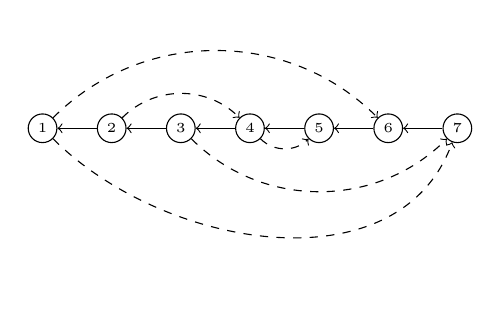
\begin{tikzpicture}[node distance = 0.5cm, inner sep = 2pt]
\tikzstyle{every node}=[circle, draw]
\tiny
\node (1) {1};
\foreach \i in {2,3,4,5,6,7} {
	\pgfmathtruncatemacro{\x}{\i-1};
	\node (\i) [right= of \x] {\i};
	\draw[->] (\i) -- (\x);
}
\small
\tikzstyle{every node}=[]
\draw[->, dashed] (1)
	edge [out = 45, in=-225] node [above] {} (6)
	edge [out=-45, in = 250] node [below] {} (7);
\draw[->, dashed] (2) edge [out = 45, in=-225] node [above] {} (4);
\draw[->, dashed] (3) edge [out = -45, in = 225] node [below] {} (7);
\draw[->, dashed] (4) edge [out = -45, in = 225] node [below] {} (5);
\end{tikzpicture}
\end{minipage}
\hfill
\begin{minipage}{0.4\linewidth}
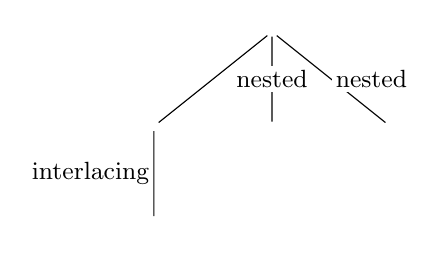
\begin{tikzpicture}[inner sep= 1.5pt]
\small
 \node {}
 [level distance = 12mm]
    child {
    	node {}
    	child {
        	node {}
        	edge from parent node[left, fill = white] {interlacing}
        }
        edge from parent node[left] {}
    }
    child {
    	node {}
    	edge from parent node[midway, fill = white] {nested}
    }
    child {
    	node {}
    	edge from parent node[right, fill = white] {nested}
    };
\end{tikzpicture}
\end{minipage}
\caption{
The left side of the figure shows a DFS tree with a chain decomposition; tree-edges are solid and back-edges are dashed.  is (\edge{1}{6},\edge{6}{5},\edge{5}{4},\edge{4}{3},\edge{3}{2},\edge{2}{1}),  is (\edge{1}{7},\edge{7}{6}),  is (\edge{2}{4}),  is (\edge{3}{7}), and  is (\edge{4}{5}).  and  are nested children of  and  is an interlacing child of . Also,  s-belongs to .} \label{fig:chains}
\end{figure}

We call  a \emph{chain decomposition}. It can be computed in time . For 2-edge-connected graphs the term decomposition is justified by Lemma~\ref{lem:2connectivity}.

\begin{lemma}[\cite{Schmidt2013a}]\label{lem:2connectivity}
Let  be a chain decomposition of a graph . Then  is 2-edge-connected if and only if  is connected and the chains in  partition .
\end{lemma}

Since the condition of Lemma~\ref{lem:2connectivity} is easily checked during the chain decomposition, we assume from now on that  is 2-edge-connected. Then  partitions  and the first chain  is a cycle containing  (since there is a back-edge incident to ). We say that  \emph{strongly belongs (s-belongs)} to the first chain and any vertex  \emph{s-belongs} to the chain containing the edge . We use s-belongs instead of belongs since a vertex can belong to many chains when chains are viewed as sets of vertices.

We can now define a parent-tree on chains. The first chain  is the root. For any chain , let the \emph{parent}  of  be the chain to which  s-belongs. We write  () for chains  and  if  is an ancestor (proper ancestor) of  in the parent-tree on chains.

The following lemma summarizes important properties of chain decompositions.

\begin{lemma}\label{facts about chain decomposition}
Let  be a chain decomposition of a 2-edge-connected graph  and let  be the root of the DFS-tree. Then
\begin{compactenum}[(1)]
\item \label{s not above t} For every chain , .
\item \label{properties of parent chain} Every chain , , has a parent chain . We have  and  for some .
\item \label{t-parent precedes t} For : If , . If , .
\item \label{parent on chains follows parent on nodes} If ,  s-belongs to , and  s-belongs to  then .
\item \label{t(D) above u} If  and  s-belongs to , then .
\item \label{s(C) s-belongs to earlier chain} For :  s-belongs to a chain  with .
\end{compactenum}
\end{lemma}
\begin{proof}
(\ref{s not above t}) to (\ref{t-parent precedes t}) follow from the discussion preceding the Lemma and the construction of the chains. We turn to (\ref{parent on chains follows parent on nodes}). Consider two vertices  and  with  and let  s-belong to  and let  s-belong to . Then , as the following simple induction on the length of the tree path from  to  shows. If ,  by the definition of s-belongs. So assume  is a proper ancestor of . Since  s-belongs to , by definition  and  is contained in . Let  be the chain to which  s-belongs. By induction hypothesis, . Also, either  (if  s-belongs to ) or  (if ) and hence  s-belongs to . In either case .

Claim (\ref{t(D) above u}) is an easy consequence of (\ref{parent on chains follows parent on nodes}). If , , and the claim follows. If ,  s-belongs to . Thus,  by  (\ref{parent on chains follows parent on nodes}).

The final claim is certainly true for each  with . So assume  and let . Since  is 2-edge-connected, there is a back-edge  with  and . It induces a chain  with  and hence  is contained in a chain  with . \qed
\end{proof}



\section{Chains as Mader-paths}\label{Chains as Mader-paths}

We show that, assuming that the input graph is 3-edge-connected, there are two chains that form a subdivision of a , and that the other chains of the chain decomposition can be added one by one such that each chain is a Mader-path with respect to the union of the previously added chains. We will also show that chains can be added parent-first, i.e., when a chain is added, its parent was already added. In this way the current graph  consisting of the already added chains is always \emph{parent-closed}. We will later show how to compute this ordering efficiently. We will first give an  algorithm and then a linear time algorithm.




Using the chain decomposition, we can identify a  subdivision in the graph as follows. We may assume that the first two back-edges explored from  in the DFS have their other endpoint in the same subtree  rooted at some child of . The first chain  forms a cycle. The vertices in  are then contained in . By assumption, the second chain is constructed by another back-edge that connects  with a vertex in . If there is no such back-edge, the tree edge connecting  and the root of  and the back edge from  into  form a -edge cut. 
Let . Then  forms a  subdivision with branch vertices  and . The next lemma derives properties of parent-closed unions of chains.

\begin{lemma}\label{parent-closed union of chains}
Let  be a parent-closed union of chains that contains  and
. Then
\begin{compactenum}[(1)]
\item For any vertex  of , the edge  is contained in , i.e., the set of vertices of  is a parent-closed subset of the DFS-tree.
\item  and  are branch vertices of  for every chain  contained in .
\item Let  be a chain that is not in  but a child of some chain in . Then  is an ear with respect to  and the path  is contained in .  is a Mader-path (i.e., the endpoints of  are not inner vertices of the same link of ) with respect to  if and only if there is a branch vertex on .
\end{compactenum}
\end{lemma}
\begin{proof}
(1): Let  be any vertex of . Let  be a chain in  containing the vertex . If  also contains  we are done. Otherwise,  or . In the first case,  s-belongs to , in the second case  s-belongs to some  by Lemma~\ref{facts about chain decomposition}.(\ref{parent on chains follows parent on nodes}). Hence, by parent-closedness,  is an edge of .

(2): Let  be any chain in . Since  and  form a ,  and  are branch vertices. If , the edge  is in  by (1), the back-edge  inducing  is in , and the path  is in  by (1). Thus  has degree at least three. If , let  be the chain to which  s-belongs, i.e.  is the parent of . As  is parent-closed  is contained in . By the definition of s-belongs,  has degree two on the chain . Further, it has degree one on the chain . Since chains are edge-disjoint, it has degree at least three in .


(3) We first observe that  and  belong to . For , this holds since  s-belongs to  and  is part of  by assumption. For , this follows from  and (1). No inner vertex  of  belongs to , because otherwise the edge  would belong to  by (1), which implies that  would belong to , as  is a union of chains. Thus  is an ear with respect to , i.e., it is disjoint from  except for its endpoints. Moreover, the path  belongs to  by (1).

If there is no branch vertex on , the vertices  and  are inner vertices of the same link of  and hence  is not a Mader-path with respect to . If there is a branch vertex on , the vertices  and  are inner vertices of two distinct links of  and hence  is a Mader-path with respect to .
\qed
\end{proof}

We can now prove that chains can always be added in parent-first order. For a link , each edge in  that is incident to an end vertex of  is called an \emph{extremal} edge of .

\begin{theorem}\label{order exists} Let  be a graph and let  be a parent-closed union of chains such that no child of a chain  is a Mader-path with respect to  and there is at least one such chain. Then the extremal edges of every link of length at least two in  are a 2-cut in .
\end{theorem}
\begin{proof} Assume otherwise. Then there is a parent-closed union  of
  chains such that no child of a chain in  is a Mader-path with respect to  and there is at least one such chain outside of , but for every link in  the extremal edges are not a cut in .

Consider any link  of . Since the extremal edges of  do not form a 2-cut, there is a path in  connecting an inner vertex on  with a vertex that is either a branch vertex of  or a vertex on a link of  different from . Let  be such a path of minimum length. By minimality, no inner vertex of  belongs to . Note that  is a Mader-path with respect to . We will show that at least one edge of  belongs to a chain  with  and that  can be added, contradicting our choice of .

Let  and  be the endpoints of , and let  be the lowest common ancestor of all points in . Since a DFS generates only tree- and back-edges,  lies on . Since  and the vertex set of  is a parent-closed subset of the DFS-tree,  belongs to . Thus  cannot be an inner vertex of  and hence is 
equal to  or . Assume w.l.o.g.~that . All vertices of  are descendants of . We view  as oriented from  to .

Since  is a vertex of , the path  is part of  by Lemma~\ref{facts about chain decomposition} and hence no inner vertex of  lies on this path. Let  be the first edge on . The vertex  must be a descendant of  as otherwise the path  would contain a cross-edge, i.e.\ an edge between different subtrees. Hence  is a back-edge. Let  be the chain that starts with the edge .  does not belong to , as no edge of  belongs to .

We claim that  is a proper descendant of  or  is a Mader-path with respect to . Since  is a descendant of  and  is an ancestor of ,  is either a proper descendant of , equal to , or a proper ancestor of . We consider each case separately.

If  were a proper ancestor of  the edge  would belong to  and hence  would be part of , contradicting our choice of . If  is equal to  then  is a Mader-path with respect to . This leaves the case that  is a proper descendant of .

Let  be the last edge on the path  that is not in  and let  be the chain containing . Then  by Lemma~\ref{facts about chain decomposition}.(\ref{t(D) above u}) (applied with  and ) and hence  by part (\ref{parent on chains follows parent on nodes}) of the same lemma. Also . Since , .

As  and  are not inner vertices of the same link, the path  contains a branch vertex. Thus  is a Mader-path by Lemma~\ref{parent-closed union of chains}.
\qed
\end{proof}
\begin{corollary}\label{greedy works}  If  is 3-edge-connected, chains can be greedily added in parent-first order.
\end{corollary}
\begin{proof} If we reach a point where not all chains are added, but we can not proceed in a greedy fashion, by Theorem~\ref{order exists} we find a cut in .
\end{proof}

\section{A First Algorithm}\label{A First Algorithm}

Corollary~\ref{greedy works} gives rise to an  algorithm, the Greedy-Chain-Addition Algorithm. In addition to , we maintain the following data structures:
\newcommand{\cL}{\ensuremath{\mathcal{L}}\xspace}
\begin{compactitem}
\item The current graph . Each link is maintained as a doubly linked list of vertices. Observe that all inner vertices of a link lie on the same tree path and hence are numbered in decreasing order. The vertices in  are labeled \emph{inactive}, \emph{branch}, or \emph{non-branch}. The vertices in  are called \emph{inactive}. Every non-branch vertex stores a pointer to the link on which it lies and a list of all chains incident to it and having the other endpoint as an inner vertex of the same link. \item A list \cL of addable chains. A chain is addable if it is a Mader-path with respect to the current graph.
\item For each chain its list of children.
\end{compactitem}

We initialize  to . It has three links, , , and . We then iterate over the children of  and . For each child, we check in constant time whether its endpoints are inner vertices of the same link. If so, we associate the chain with the link by inserting it into the lists of both endpoints. If not, we add the chain to the list of addable chains. The initialization process takes time .

As long as the list of addable chains is non-empty, we add a chain, say . Let  and  be the endpoints of . We perform the following actions:
\begin{compactitem}
\item If  is a non-branch vertex, we make it a branch vertex. This splits the link containing it and entails some processing of the chains having both endpoints on this link.
\item If  is a non-branch vertex, we make it a branch vertex. This splits the link containing it, and entails some processing of the chains having both endpoints on this link.
\item We add  as a new link to .
\item We process the children of .
\end{compactitem}
We next give the details for each action.

If  is a non-branch vertex, it becomes a branch vertex. Let  be the link of  containing ;  is split into links  and  and the set  of chains having both endpoints on  is split into sets ,  and , where  is the set of chains having both endpoints on , , and  is the set of chains that become addable (because they are incident to  or have one endpoint each in  and ). We show that we can perform the split of  in time . We walk from both ends of  towards  in lockstep fashion. In each step we either move to the next vertex or consider one chain. Once we reach  we stop. Observe that this strategy guarantees the time bound claimed above.

When we consider a chain, we check whether we can move it to the set of addable chains. If so, we do it and delete the chain from the lists of both endpoints. Once, we have reached , we split the list representing the link into two. The longer part of the list retains its identity, for the shorter part we create a new list header and redirect all pointers of its elements.

Adding  to  is easy. We establish a list for the new link and let all inner vertices of  point to it. The inner vertices become active non-branch vertices.

Processing the children of  is also easy. For each child, we check whether both endpoints are inner vertices of . If so, we insert the child into the list of its endpoints. If not, we add the child to the list of addable chains.


If \cL becomes empty, we stop. If all chains have been added, we have constructed a Mader sequence. If not all chains have been processed, there must be a link having at least one inner vertex. The first and the last edge of this link form a 2-edge-cut.

It remains to argue that the algorithm runs in time . We only need to argue about the splitting process. We distribute the cost  as follows:  is charged to the vertex that becomes a branch vertex. All such charges add up to .  is charged to the chains that become addable. All such charges add up to .  is charged to the vertices and chains that define the minimum. We account for these charges with the following token scheme inspired by the analysis of the corresponding recurrence relation in~\cite{Me3}.


Consider a link  with  chains having both endpoints on . We maintain the invariant that each vertex and chain owns at least  tokens. When a link is newly created we give  tokens to each vertex of the link and to each chain having both endpoints on the link. In total we create  tokens. Assume now that we split a link  with  chains into links  and  with  and  chains respectively. Then  and hence we may take one token away from each vertex and chain of the sublink that is charged without violating the token invariant.

\begin{theorem} The Greedy-Chain-Addition algorithm runs in time .
\end{theorem}

\section{A Classification of Chains}\label{A Classification of Chains}
When we add a chain in the Greedy-Chain-Addition algorithm, we also process its children. Children that do not have both endpoints as inner vertices of the chain can be added to the list of addable chains immediately. However, children that have both endpoints as inner vertices of the chain cannot be added immediately and need to be observed further until they become addable. We now make this distinction explicit by classifying chains into two types, interlacing and nested.

We classify the chains  into two types. Let  be a chain with parent . We distinguish two cases\footnote{In~\cite{Schmidt2013}, three types of chains are distinguished. What we call nested is called Type 1 there and what we call interlacing is split into Types 2 and 3 there. We do not need this finer distinction.} for .
\begin{compactitem}
	\item If  is an ancestor of  and a descendant of ,  is \emph{interlacing}. We have .
	\item If  is a proper descendant of ,  is \emph{nested}. We have  and  is contained in .
\end{compactitem}
These cases are exhaustive as the following argument shows. Let  be the first edge on . By Lemma~\ref{facts about chain decomposition}, . We split the path  into  and . Depending on which of these paths  lies on,  is interlacing or nested.

The following simple observations are useful. For any chain ,  s-belongs to . If  is nested,  and  s-belong to . If  is interlacing,  s-belongs to a chain which is a proper ancestor of  or . The next lemma confirms that interlacing chains can be added once their parent belongs to .

\begin{lemma}\label{interlacing are easy}
Let  be a parent-closed union of chains that contains  and , let  be any chain contained in , and let  be an interlacing child of  not contained in . Then  is a Mader-path with respect to .
\end{lemma}
\begin{proof} We have already shown in Lemma~\ref{parent-closed union of chains} that  is an ear with respect to , that the path  is part of , and that  and  are branching vertices of . Since  is interlacing, we have . Thus  contains a branching vertex and hence  is a Mader-path by Lemma~\ref{parent-closed union of chains}.(3). \qed
\end{proof}

\section{A Linear Time Algorithm}\label{sec:linear time alg}


According to Lemma~\ref{interlacing are easy}, interlacing chains whose parent belongs to the current graph are always Mader-paths and can be added. Nested chains have both endpoints on their parent chain and can only be added once the tree-path connecting its endpoints contains a branching point. Consider a chain nested in chain . Which chains can help its addition by creating branching points on ? First,  interlacing chains having their source on some  with , and second, chains nested in  and their interlacing offspring having  their source on . Chains having their source on some  with  cannot help because they have no endpoint on . This observation shows that chains can be added in phases. In the -th phase, we try to add all chains having their source vertex on .







\begin{algorithm}[t]
\caption{Certifying linear-time algorithm for 3-edge connectivity.}\label{alg: main}
\begin{algorithmic}
\Procedure{Connectivity}{G=(V,E)}
\State Let  be a chain decomposition of  as
described in Sect.~\ref{sec:chain decomposition};
\State Initialize  to ;
\For { from 1 to }
             \Comment \emph{Phase : add all chains whose source s-belongs to }
	\State Group the chains  for which  s-belongs to  into
        segments;
\State \emph{Part I of Phase }: Add all segments to  whose minimal chain is interlacing;
	\State \emph{Part II of Phase }: Either find an insertion order  of the segments having a nested minimal chain or exhibit a 2-edge-cut and stop;
	\For { from 1 to }
		\State Add the chains contained in  parent-first;
	\EndFor
\EndFor
\EndProcedure
\end{algorithmic}
\end{algorithm}

The overall structure of the linear-time algorithm is given in Algorithm~\ref{alg: main}. An implementation in Python is available at \url{https://github.com/adrianN/edge-connectivity}. The algorithm operates in phases and maintains a current graph . Let , , \ldots,  be the chains of the chain decomposition in the order of creation. We initialize  to . In phase , , we consider the -th chain  and either add all chains  to  for which the source vertex  s-belongs to  to  or exhibit a 2-edge-cut. As already mentioned, chains are added parent-first and hence  is always parent-closed. We maintain the following invariant:\smallskip

\noindent{\textbf{Invariant:}} After phase ,  consists of all chains for which the source vertex s-belongs to one of the chains  to .

\begin{lemma}\label{prop:ci_already_added}
For all , the current chain  is part of the current graph  at the beginning of phase  or the algorithm has exhibited a 2-edge-cut before phase .
\end{lemma}
\begin{proof}
The initial current graph consists of chains  and  and hence the claim is true for the first and the second phase. Consider . The source vertex  s-belongs to a chain  with  (Lemma~\ref{facts about chain decomposition}.(\ref{s(C) s-belongs to earlier chain})) and hence  is added in phase . \qed
\end{proof}

The next lemma gives information about the chains for which the source vertex s-belongs to . None of them belongs to  at the beginning of phase  (except for chain  that belongs to  at the beginning of phase ) and they form subtrees of the chain tree. Only the roots of these subtrees can be nested. All other chains are interlacing.

\begin{lemma}\label{lem:no_type_one} Assume that the algorithm reaches phase  without exhibiting a 2-edge-cut. Let  be a chain for which  s-belongs to . Then  is not part of  at the beginning of phase . Let  be any ancestor of  that is not in . Then:
\begin{compactenum}[(1)]
\item  s-belongs to .
\item If  is nested, it is a child of .
\item If  is not part of the current graph,  is interlacing.
\end{compactenum}
\end{lemma}
\begin{proof}
We use induction on . Consider the -th phase and let  be chains whose source vertex  s-belongs to . We first prove that  is not in . This is obvious, since in the -th phase we add exactly the chains whose source vertex -belongs to .

(1): Let  be any ancestor of  which is not part of . By Lemma~\ref{facts about chain decomposition}, we have  and hence  belongs to  for some . If ,  would have been added in phase , a contradiction to the assumption that  does not belong to  at the beginning of phase .

(2):  s-belongs to  by (1). If  is nested,  and  s-belong to the same chain. Thus  is a child of .

(3): If  is not part of the current graph,  by Lemma~\ref{prop:ci_already_added} and hence  is not a child of . Hence by (2),  is interlacing.\qed
\end{proof}

We can now define the segments with respect to  by means of an equivalence relation. Consider the set  of chains whose source vertex s-belongs to . For a chain , let  be the minimal ancestor of  that does not belong to . Two chains  and  in  belong to the same segment if and only if . In Figure~\ref{fig:chains} on page~\pageref{fig:chains}, if we start with , we form three segments in the first phase, namely , , and . The first segment can be added according to Lemma~\ref{interlacing are easy}. Then  can be added and then .

Consider any . By part (1) of the preceding lemma either  or  is part of . Moreover,  and  belong to the same segment in the first case. Thus segments correspond to subtrees in the chain tree. In any segment only the minimal chain can be nested by Lemma~\ref{lem:no_type_one}. If it is nested, it is a child of  (parts (2) and (3) of the preceding lemma). Since only the root of a segment may be a nested chain, once it is added to the current graph all other chains in the segment can be added in parent-first order by Lemma~\ref{interlacing are easy}. All that remains is to find the proper ordering of the segments faster than in the previous section. We do so in Lemma~\ref{lem:add_hard_segments}. If no proper ordering exists, we exhibit a 2-edge-cut.








\begin{lemma}\label{cor:add_segment} All chains in a segment  can be added in parent-first order if its minimal chain can be added.
\end{lemma}
\begin{proof} By Lemma~\ref{lem:no_type_one} all but the minimal chain in a segment are interlacing. Thus the claim follows from Lemma~\ref{interlacing are easy}. \qed
\end{proof}

We come to part I of phase , the addition of all segments whose minimal chain is interlacing. As a byproduct, we will also determine all segments with nested minimal chain. We iterate over all chains  whose source  s-belongs to . For each such chain, we traverse the path , , , \ldots until we reach a chain that belongs to  or is already marked (initially, all chains are unmarked). We now distinguish cases. If the last chain on the path is nested we mark all chains on the path with the nested chain. If we hit a marked chain we copy the marker to all chains in the path.  Otherwise, i.e., all chains are interlacing and unmarked, we add all chains in the path to  in parent-first order, as these segments can be added according to Corollary~\ref{cor:add_segment}. 

It remains to compute a proper ordering of the segments in which the minimal chain is nested or to exhibit a 2-edge-cut. We do so in part II of phase . For simplicity, we will say `segment' instead of `segment with nested minimal chain' from now on.

For a segment  let the \emph{attachment points} of  be all vertices in  that are in . Note that the attachment points must necessarily be endpoints of chains in  and hence adding the chains of  makes the attachment points branch vertices. Nested children  of  can be added if there are branch vertices on , therefore adding a segment can make it possible to add further segments.

\begin{lemma}\label{prop:attachment points} Let  be a nested child of  and let  be the segment containing . The attachment points of  consist of , , and the vertices  of the other chains in the segment. All such points lie on the path  and hence on . \end{lemma} 
\begin{proof} Let  be any chain in  different from . By Lemma~\ref{lem:no_type_one},  is the minimal chain in . Since  is a subtree of the chain tree, we have  and hence by Lemma~\ref{facts about chain decomposition} . Since none of the chains in  is part of , parent-closedness implies that no vertex on the path  belongs to . In particular, either  or  is not a vertex of  and hence not an attachment point of . It remains to show . Since , we have  by Lemma~\ref{facts about chain decomposition}. Since  and  we have either  or . In the former case, we are done. In the latter case,  is not a vertex of  by the preceding paragraph, a contradiction, since  s-belongs to  by Lemma~\ref{lem:no_type_one}.
\qed
\end{proof}

For a set of segments , let the \emph{overlap graph} be the graph on the segments and a special vertex  for the branch vertices on . In the overlap graph, there is an edge between  and a vertex , if there are attachment points  of  such that there is a branch vertex on the tree path . Further, between two vertices  and  there is an edge if there are attachment points ,  in  and ,  in , such that  or . We say that  and  \emph{overlap}.

\newcommand{\calC}{{\mathcal{C}}}

\begin{lemma}\label{overlap with calC suffices}
Let  be a connected component of the overlap graph  and let  be any segment with respect to  whose minimal chain  is nested. Then  if and only if
  \begin{compactenum}[(i)]
  \item \label{connected by branch}  and there is a branch vertex on  or
  \item \label{connected by overlap} there are attachments  and  of  and attachments  and  of segments in  with  or .
  \end{compactenum}
\end{lemma}
\begin{proof} We first show  if (\ref{connected by branch}) or (\ref{connected by overlap}) holds. For (\ref{connected by branch}) the claim follows directly from the definition of the overlap graph. For (\ref{connected by overlap}), assume  for the sake of a contradiction. Then either  or there is no branch vertex in  by (\ref{connected by branch}). Further, no segment in  overlaps with  and hence any segment in  has its attachments points either strictly between  and  or outside the path . Moreover, both classes of segments are non-empty. However, segments in the two classes do not overlap and  cannot be connected to the segments in the former class. Thus  is not connected, a contradiction.

If neither (\ref{connected by branch}) nor (\ref{connected by overlap}) hold, there can be no segment in  overlapping  and either  is not connected to  or no segment in  is connected to .
\end{proof}


\begin{lemma}\label{lem:add_hard_segments}
  Assume the algorithm reaches phase . If the overlap graph  induced by the segments with respect to   is connected, we can add all segments of . If  is not connected, we can exhibit a 2-edge-cut for any component of  that does not contain .
\end{lemma}
\begin{proof} Assume first that  is connected. Let  be the vertices of  in a preorder, e.g.\ the order they are explored by a DFS, starting at , the vertex corresponding to the branch vertices on . An easy inductive argument shows that we can add all segments in this order. Namely, let  and let  be the minimal chain of . All attachment points of  lie on the path  by Lemma~\ref{prop:attachment points}, and there is either an edge between  and  or an edge between  and  for some .  In the former case, there is a branch vertex on  at the beginning of the phase, in the latter case there is one after adding . Thus the minimal chain of  can be added and then all other chains by Lemma~\ref{cor:add_segment}.

On the other hand, suppose  is not connected. Let  be any connected component of  that does not contain , and let  be the connected component that contains . Let  and  be the minimal and maximal attachment points of the segments in , and let  be the current graph after adding all chains in . We first show that there is no branch vertex of  on the path . Assume otherwise and let  be any such branch vertex. Observe first that there must be a chain  with . Otherwise, every chain in  has all its attachment points at proper ancestors of  or at proper descendants of  and hence  is not connected. Let  be the segment containing . By Lemma~\ref{prop:attachment points}, we may assume that  is the minimal chain of . Since ,  is not an edge of  and hence no branch vertex exists on the path  at the beginning of part II of the phase. Hence  is an attachment point of a segment in . In particular  contains at least one segment. We claim that  must also have an attachment point outside . This holds since all initial branch vertices are outside the path and since  is connected. Thus  by Lemma~\ref{overlap with calC suffices},  a contradiction.

We show next that the tree-edge  and the edge  from 's predecessor  on  to  form a 2-edge-cut;  may be a tree-edge or a back-edge. The following argument is similar to the argument in Theorem~\ref{order exists}, but more refined.

Assume otherwise. Then, as in the proof of Theorem~\ref{order exists}, there is a path  such that  for all , and either  lies on  and  does not, or vice versa, and no inner vertex of  is in . Moreover, the first edge  of  is a back-edge and  is a descendant of . Note that unlike in the proof of  Theorem~\ref{order exists},  and  need not lie on different links, as we want to show that  and  form a cut and these might be different from the last edges on the link containing  and .

Let  be the chain that starts with the edge .  does not belong to , as no edge of  belongs to . In particular,  does not s-belong to  for  (as otherwise,  would already be added). Since  and one of  and  lies on  (which is a subpath of ),  s-belongs to . By the argument from the proof of Theorem~\ref{order exists},  is a descendant of .

Let  be the chain that contains the last edge of . If , . Otherwise,  is a proper descendant of . Let  be the last edge on the path .  We claim that  is also the last edge of . This holds since the last edge of  must come from a descendant of  (as ancestors of  belong to ) and since it cannot come from a child different from  as otherwise  would have to contains a cross-edge. Thus  by Lemma~\ref{facts about chain decomposition}.(\ref{t(D) above u}) and hence  by part (\ref{parent on chains follows parent on nodes}) of the same lemma.

 and  belong to the same segment with respect to , say , and  and  are vertices in . This can be seen easily. Since  s-belongs to ,  belongs to some segment with respect to  and since ,  belongs to the same segment. Since  and  is a vertex of ,  is the minimal chain in . Thus  is nested and hence  s-belongs to . Hence  and  are attachment points of .

Thus  overlaps with  and hence  by Lemma~\ref{overlap with calC suffices}. Therefore  and  are not the extremal attachment points, that is the minimal (or maximal) vertices in , of , a contradiction. \qed
\end{proof}


It remains to show that we can find an order as required in Lemma~\ref{lem:add_hard_segments}, or a 2-edge-cut, in linear time. We reduce the problem of finding an order on the segments to a problem on intervals. W.l.o.g.\ assume that the vertices of  are numbered consecutively from  to . Consider any segment , and let  be the set of attachment points of , i.e., the set of vertices that  has in common with . By Lemma~\ref{prop:attachment points},  and  are the endpoints of the minimal chain in  and each , , is equal to  for some other chain in . We associate the intervals
with  and for every branch vertex  on  we define an interval . See Figure~\ref{fig:attachment_point_intervals} for an example.
\begin{figure}
\centering
\definecolor{cffffff}{RGB}{255,255,255}
\definecolor{c0000ff}{RGB}{0,0,255}
\begin{tikzpicture}[y=0.60pt, x=0.6pt,yscale=-1, inner sep=0pt, outer sep=0pt]
    \path[shift={(0,1.66744)},fill=black]
      (134.8939,81.4960)arc(0.000:180.000:4.000)arc(-180.000:0.000:4.000) -- cycle;
    \path[draw=black,dashed,line join=miter,line cap=butt,line width=0.800pt]
      (159.4488,83.1635) -- (302.2232,83.1635) .. controls (302.2232,83.1635) and
      (248.3759,41.0607) .. (216.5586,41.0607) .. controls (184.7413,41.0607) and
      (130.8939,83.1635) .. (130.8939,83.1635);
    \path[fill=black] (154.84824,98.587296) node[above right] (text3027) {};
    \path[fill=black] (202.43971,98.587296) node[above right] (text3031) {};
    \path[fill=black] (250.03119,98.587296) node[above right] (text3035) {};
    \path[fill=black] (297.62265,98.587296) node[above right] (text3039) {};
    \path[shift={(2.01483,-1.25057)},draw=black,fill=cffffff]
      (256.6169,84.4141)arc(0.000:180.000:4.000)arc(-180.000:0.000:4.000) -- cycle;
    \path[fill=black] (416.13892,98.587296) node[above right] (text3027-8) {};
    \path[fill=black] (458.60425,98.587296) node[above right] (text3031-6) {};
    \path[fill=black] (500.96216,98.587296) node[above right] (text3035-9) {};
    \path[fill=black] (543.7937,98.587296) node[above right] (text3039-1) {};
    \path[fill=black] (373.78101,98.728889) node[above right] (text4128) {};
    \path[draw=black,line join=miter,line cap=butt,line width=0.800pt]
      (374.9402,41.6045) -- (417.2375,41.6045);
    \path[draw=black,line join=miter,line cap=butt,line width=0.800pt]
      (417.2375,39.6244) -- (417.2375,43.5846);
    \path[draw=black,line join=miter,line cap=butt,line width=0.800pt]
      (374.9402,39.6244) -- (374.9402,43.5846);
    \path[draw=black,line join=miter,line cap=butt,line width=0.800pt]
      (374.9402,39.6244) -- (374.9402,43.5846);
    \path[draw=c0000ff,line join=miter,line cap=butt,line width=0.800pt]
      (159.4488,83.1635) .. controls (163.8978,75.9450) and (248.9835,20.3629) ..
      (285.2178,38.3891) .. controls (295.8598,60.2515) and (302.2232,83.1635) ..
      (302.2232,83.1635);
    \path[draw=c0000ff,line join=miter,line cap=butt,line width=0.800pt]
      (207.0403,83.1635) .. controls (232.2578,58.7003) and (258.3328,43.9550) ..
      (285.2178,38.3891);
    \path[shift={(15.70172,1.25058)},draw=black,fill=cffffff]
      (195.3386,81.9129)arc(0.000:180.000:4.000)arc(-180.000:0.000:4.000) -- cycle;
    \path[shift={(32.86245,-45.85455)},draw=black,fill=cffffff]
      (256.6169,84.4141)arc(0.000:180.000:4.000)arc(-180.000:0.000:4.000) -- cycle;
    \path[shift={(-1.04214,1.25058)},fill=black]
      (164.4910,81.9129)arc(0.000:180.000:4.000)arc(-180.000:0.000:4.000) -- cycle;
    \path[draw=black,fill=cffffff]
      (306.2232,83.1635)arc(0.000:180.000:4.000)arc(-180.000:0.000:4.000) -- cycle;
    \path[draw=black,line join=miter,line cap=butt,line width=0.800pt]
      (417.2376,81.8313) -- (544.2820,81.8313);
    \path[draw=black,line join=miter,line cap=butt,line width=0.800pt]
      (544.2820,79.8512) -- (544.2820,83.8114);
    \path[draw=black,line join=miter,line cap=butt,line width=0.800pt]
      (417.2376,79.8512) -- (417.2376,83.8114);
    \path[draw=black,line join=miter,line cap=butt,line width=0.800pt]
      (417.2376,79.8512) -- (417.2376,83.8114);
    \path[draw=black,line join=miter,line cap=butt,line width=0.800pt]
      (417.2376,68.4224) -- (459.3367,68.4224);
    \path[draw=black,line join=miter,line cap=butt,line width=0.800pt]
      (459.3367,66.4423) -- (459.3367,70.4025);
    \path[draw=black,line join=miter,line cap=butt,line width=0.800pt]
      (417.2376,66.4423) -- (417.2376,70.4025);
    \path[draw=black,line join=miter,line cap=butt,line width=0.800pt]
      (417.2376,66.4423) -- (417.2376,70.4025);
    \path[draw=black,line join=miter,line cap=butt,line width=0.800pt]
      (459.6248,55.0134) -- (544.2820,55.0134);
    \path[draw=black,line join=miter,line cap=butt,line width=0.800pt]
      (544.2820,53.0334) -- (544.2820,56.9935);
    \path[draw=black,line join=miter,line cap=butt,line width=0.800pt]
      (459.6248,53.0334) -- (459.6248,56.9935);
    \path[draw=black,line join=miter,line cap=butt,line width=0.800pt]
      (459.6248,53.0334) -- (459.6248,56.9935);
\end{tikzpicture}
\caption{Intervals for the solid segment with respect to the dashed chain. It has the attachment points ,,. Filled vertices are branching points.}
\label{fig:attachment_point_intervals}
\end{figure}

We say two intervals  \emph{overlap} if . Note that overlapping is different from intersecting; an interval does not overlap intervals in which it is properly contained or which it properly contains. This relation naturally induces a graph  on the intervals. Contracting all intervals that are associated to the same segment into one vertex makes  isomorphic to the overlap graph as required for Lemma~\ref{lem:add_hard_segments}. Hence we can use  to find the order on the segments. Note that the interval set  for each segment does not suffice without employing a clever tie-breaking rule: If there are two segments with attachments  and , respectively, such that , no interval of the first segment overlaps with one of the second.

A naive approach that constructs , contracts intervals, and runs a DFS will fail, since the overlap graph can have a quadratic number of edges. However, using a method developed by Olariu and Zomaya~\cite{Olariu1996}, we can compute a spanning forest of  in time linear in the number of intervals. The presentation in~\cite{Olariu1996} is for the PRAM and thus needlessly complicated for our purposes. A simpler explanation can be found in the appendix.

The number of intervals created for a chain  is bounded by

where  are the nested children of ,  are the interlacing chains that start on , and  is the set of branch vertices on . Note that we generate 
the interval  for each nested child , and the intervals  and  for each interlacing chain  belonging to a segment with nested minimal chain . Thus the total time spend the ordering procedure is . 
From the above discussion, we get:

\begin{theorem}
For a -edge-connected graph, a Mader construction sequence can be found in time O().
\end{theorem}


\section{Verifying the Mader Sequence}\label{sec:verify mader}

The certificate is either a 2-edge-cut, or a sequence of Mader-paths. For a 2-edge-cut, we simply remove the two edges and verify that  is no longer connected.

For checking the Mader sequence, we doubly-link each edge in a Mader-path to the corresponding edge in . Let  be a copy of . We remove the Mader-paths, in reverse order of the sequence, suppressing vertices of degree two as they occur. This can create multiple edges and loops. Let  be the multi-graph before we remove the -th path . We need to verify the following:

\begin{compactitem}
\item  must have minimum degree three.
\item The union of Mader-paths must be isomorphic to  and the Mader-paths must partition the edges of . This is easy to check using the links between the edges of the paths and the edges of .
\item The paths we remove must be ears. More precisely, at step ,  must have been reduced to a single edge in , as inner vertices of  must have been suppressed if  is an ear for .
\item The  must not subdivide the same link twice. That is, after deleting the edge corresponding to , it must not be the case that both endpoints are still adjacent (or equal, i.e.\  is a loop) but have degree two.
\item When only two paths are left, the graph must be a .
\end{compactitem}




\section{The Cactus Representation of 2-Cuts}\label{Sec: Cactus Representation}
We review the cactus representation of 2-cuts in a 2-connected but not 3-connected graph and show how to certify it.

A \emph{cactus} is a graph in which every edge is contained in exactly one cycle. Dinits, Karzanov, and Lomonsov~\cite{Dinits-Karzanov-Lomonosov} showed that the set of mincuts of any graph has a cactus representation, i.e., for any graph  there is a cactus  and a mapping  such that the mincuts of  are exactly the preimages of the mincuts of , i.e., for every mincut\footnote{For this theorem, a cut is specified by a set of vertices, and the edges in the cut are the edges with exactly one endpoint in the vertex set.} ,  is a mincut of , and all mincuts of  can be obtained in this way. The pair  is called a \emph{cactus representation} of . Fleiner and Frank~\cite{Fleiner2009} provide a simplified proof for the existence of a cactus representation. We will call the elements of  \emph{vertices}, the elements of  \emph{nodes}, and the preimages of nodes of  \emph{blobs}.

In general, a cactus representation needs to include nodes with empty preimages. This happens for example for the ; its cactus is a star with double edges where the central node has an empty preimage and the remaining nodes correspond to the vertices of the . For graphs whose mincuts have size two, nodes with empty preimages are not needed, and a cactus representation can be obtained by contracting the 3-edge-connected components into a single node. 


\newcommand{\citeNaga}{\cite[Section 2.3.5]{Nagamochi-Ibaraki-Book}}

\begin{lemma}[\citeNaga] \label{cactus representation} Let  be a 2-edge-connected graph that is not 3-edge-connected. Contracting each 3-edge-connected components of  into a node yields a cactus representation  of  with the following properties:
\begin{compactenum}[i)]
\item The edges of  are in one-to-one correspondence to the edges of  that are contained in a 2-cut.
\item For every node ,  is a 3-edge-connected component of .
\end{compactenum}
\end{lemma}





\subsection{Verifying a Cactus Representation}

Let  be a graph and let  be an alleged cactus-representation of its 2-cuts in the sense of Lemma~\ref{cactus representation}. We show how to verify a cactus representation in linear time. We need to check two things. First, we need to ensure that  is indeed a cactus graph, that is, every edge of  is contained in exactly one cycle, that  is a surjective mapping and hence there are no empty blobs, and that every edge of  either connects two vertices in the same blob or is also present in . Second, we need to verify that the blobs of  are -edge-connected components of . For this purpose, the cactus representation is augmented by a Mader construction sequence for each blob . The verification procedure from Sect.~\ref{sec:verify mader} can then be applied.

We first verify that  is a cactus. We compute a chain decomposition of  and verify that every chain is a cycle. We label all edges in the -th cycle by . We have now verified that  is a cactus.

Surjectivity of  is easy to check. We then iterate over the edges  of . If its endpoints belong to the same blob, we associate the edge with the blob. If its endpoints do not belong to the same blob, we add the pair  to a list. Having processed all edges, we check whether the constructed list and the edge list of  are identical by first sorting both lists using radix sort and then comparing them for identity.

We finally have to check that the blobs of  correspond to 3-edge-connected components of . Our goal is to use the certifying algorithm for -edge-connectivity on the substructures of  that represent -edge-connected components. Let  be any blob. We already collected the edges having both endpoints in . We also have to account for the paths using edges outside .  We do so by creating an edge  for a every path in  leaving  at vertex  and returning to  at vertex . 
It is straightforward to compute these edges; we look at all edges having exactly one endpoint in the blob. Each such edge corresponds to an edge in . For each such edge, we know to which cycle it belongs. The outgoing edges pair up so that the two edges of each pair belong to the same cycle. 

The maximality of each blob  is given by the fact that every edge of  is contained in a 2-edge-cut of  and hence contained in a 2-edge-cut of .

Every algorithm for computing the 3-edge-connected components of a graph, e.g.~\cite{Nagamochi1992a,Taoka1992,Tsin2007,Tsin2009,Nagamochi-Ibaraki-Book}, can be turned into a certifying algorithm for computing the cactus representation of 2-cuts. We obtain the cactus  and the mapping  by contraction of the 3-edge-connected components (Lemma~\ref{cactus representation}). Then one applies our certifying algorithm for 3-edge-connectivity to each 3-edge-connected component. The drawback of this approach is that it requires  \emph{two} algorithms that check 3-connectivity. 
In the next section we will show how to extend our algorithm so that it computes the 3-edge-connected components and the cactus representation of 2-cuts of a graph directly.


\section{Computing a Cactus Representation}\label{Computing a Cactus}

We discuss how to extend the algorithm to construct a cactus representation. We begin by examining the structure of the 2-cuts of  more closely to extend our algorithm such that it finds all 2-cuts of the graph and encodes them efficiently.

We will first show that the two edges of every -edge-cut of  are contained in a common chain. This restriction allows us to focus on the -edge-cuts that are contained in the currently processed chain  only. In the subsequent section, we show how to maintain a cactus for every phase  of the algorithm that represents all -edge-cuts of the graph of the branch vertices and links of  in linear space. The final cactus will therefore represent all -edge-cuts in .

There is one technical detail regarding the computation of overlap graphs: For the computation of a Mader-sequence in Section~\ref{sec:linear time alg}, we stopped the algorithm when the first -edge-cut occurred, as then a Mader-sequence does not exist anymore. Here, we simply continue the algorithm with processing the next chain . This does not harm the search for cuts in subsequent chains, as the fact that -edge-cuts are only contained in common chains guarantees that every -edge-cut that contains an edge  in  has its second edge also in .


For simplicity, we assume that  is 2-edge-connected and has minimum degree three from now on. Then all 3-edge-connected components contain at least two vertices. 


\subsection{2-Edge-Cuts are Contained in Chains and an Efficient Representation of All Cuts in a Chain}\label{sec:efficient cut representation}

In phase  of the algorithm, using Lemma~\ref{lem:add_hard_segments}, we can find a 2-edge-cut for each connected component of the overlap graph  that does not contain  ( is the special vertex in  that represents the branch vertices on ). Lemma~\ref{lem:h induces all cuts} shows that the set of edges contained in these cuts is equal to the set of edges contained in any cut on .
Lemma~\ref{lem:facts about cuts} states easy facts about -edge-cuts, in particular, that the edges of any 2-edge-cut are contained in a common chain. The proofs can be found in many 3-connectivity papers, e.g.~\cite{Nagamochi1992a,Taoka1992,Tsin2007,Tsin2009}. As in the previous sections, all DFS-tree-edges are oriented towards the root, while back-edges are oriented away from the root.

\begin{lemma}\label{lem:facts about cuts}
Let  be a DFS-tree of a -edge-connected graph . Every -edge-cut  of  satisfies the following:

\begin{compactenum}[(1)]
  \item At least one of  and  is a tree-edge, say .\label{not both backedges}
  \item  has exactly two components. Moreover, the edges  and  have exactly one endpoint in each component.\label{endpoints disconnected}
  \item The vertices , , , and  are contained in the same leaf-to-root path of .\label{on a tree path}
  \item If  and  are tree-edges and w.l.o.g.\ , the vertices in  and  are in different components of .\label{components two tree-edges}
  \item If  is a back-edge, then  and, additionally, the vertices in  and  are in different components of .\label{components back and tree-edge}
\end{compactenum}\smallskip
\noindent Moreover, let  be a chain decomposition of . For every -edge-cut  of ,  and  are contained in a common chain .

\end{lemma}

















\begin{lemma}\label{lem:h induces all cuts}
Let  be the set of edges that are contained in the 2-edge cuts induced by the connected components of the overlap graph  at the beginning of part II of phase . Then any 2-edge-cut  on  is a subset of .
\end{lemma}
\begin{proof}
Assume for the sake of contradiction that there is an edge  in the -edge-cut that is not in . We distinguish the following cases.

First assume that both  and  are tree-edges and w.l.o.g.\ . Since  has minimal degree three, every vertex on  has an incident edge that is not on . Hence it is either a branch vertex, or belongs to some segment with respect to  (incident back-edges start chains in segments w.r.t.\ , incident tree edges are the last edges of chains in segments w.r.t.\ ). As  is a branch vertex, by Lemma~\ref{lem:facts about cuts}.(\ref{components two tree-edges}) the path  can not contain a branch vertex. In particular,  is not a branch vertex.

Let  be any segment having  as attachment vertex. All segments in the connected component of  in  must have their attachment vertices on  and the connected component does not contain . Hence this connected component induces a cut containing .

Now assume that one of  and  is a back-edge. If  is the back-edge, then  and we have  by Lemma~\ref{lem:facts about cuts}. The path  cannot contain a branch vertex. Let  be any segment that has  as attachment vertex. All segments in the connected component of  must have their attachment vertices on  and the connected component does not contain . Hence  is contained in a cut induced by this connected component.

If on the other hand  is the tree-edge we have  basically the same argument applies when we replace  by a segment  containing .
\end{proof}





We next show how to compute a space efficient representation of all 2-cuts on the chain . Using this technique we can store all 2-cuts in  in linear space. In the next section we will then use this to construct the cactus-representation of all 2-cuts in .

Number the edges in  as , , \ldots, . Here  is a back edge and  to  are tree edges. We start with a simple observation. Let . If  and  are 2-edge-cuts, then  is a 2-edge-cut.

Using this observation, we want to group the edges of -edge-cuts of  such that (i) every two edges in a group form a -edge-cut and (ii) no two edges of different groups form a -edge-cut. The existence of such a grouping has already been observed in~\cite{Nagamochi1992a,Taoka1992,Tsin2009}. We show how to find it using the data structures we have on hand during the execution of our algorithm.

Consider the overlap graph  in phase  of our algorithm. We need some notation. Let  be the set of intervals on  that contains for every component of  (except the component representing the branch vertices on ) with extremal attachment vertices  and  the interval . Since the connected components of  are maximal sets of overlapping intervals,  is a \emph{laminar family}, i.e.\ every two intervals in  are either disjoint or properly contained in each other. In particular, no two intervals in  share an endpoint.
The layers of this laminar family encode which edges form pairwise 2-cuts in , see Figure~\ref{fig:laminar family}. We define an equivalence relation to capture this intuition.

\begin{figure}
\centering
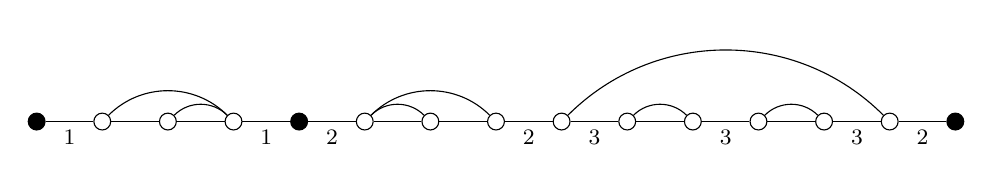
\begin{tikzpicture}[node distance=4ex]
\tikzstyle{vertex}=[circle, draw, inner sep=0.5ex]
\node[vertex, fill=black] (1) {};
\foreach \i in {2,3,4} {
  \pgfmathtruncatemacro{\left}{\i-1}
  \node[vertex, right=of \left] (\i) {};
}
\node[vertex, fill=black, right=of 4] (5) {};
\foreach \i in {6,...,14} {
    \pgfmathtruncatemacro{\left}{\i-1}
  \node[vertex, right=of \left] (\i) {};
}
\node[vertex, fill=black, right=of 14] (15) {};

\foreach \i/\j in {2/4, 3/4, 6/7, 6/8, 9/14,10/11,12/13} {
  \draw (\i) edge [out=45, in=135] (\j);
}
\foreach \i in {3,4,7,8,11,13} {
  \pgfmathtruncatemacro{\left}{\i-1}
  \draw (\i) edge (\left);
}

\footnotesize
\foreach \i in {2,5} {
  \pgfmathtruncatemacro{\left}{\i-1}
  \draw (\i) edge node [below] {1} (\left);
}
\foreach \i in {6,9,15} {
  \pgfmathtruncatemacro{\left}{\i-1}
  \draw (\i) edge node [below] {2} (\left);
}
\foreach \i in {10,12,14} {
  \pgfmathtruncatemacro{\left}{\i-1}
  \draw (\i) edge node [below] {3} (\left);
}
\end{tikzpicture}
\caption{The intervals induced by the connected components of the overlap graph  form a laminar family. The levels of this family encode which edges form pairwise 2-cuts. Two edges in the figure are labeled with the same number if they form a cut. Filled vertices are branch vertices.}
\label{fig:laminar family}
\end{figure}

For an interval , , let  and  be the edges of  directly before and after  and , respectively. We call  the \emph{interval-cut} of . For a subset  of intervals, let  be the union of edges that are contained in interval-cuts of intervals in . According to Lemma~\ref{lem:h induces all cuts}, every -edge-cut in  consists of edges in .

We now group the edges of  using the observation above. Let two intervals  and  \emph{contact} if  or . Clearly, the transitive closure  of the contact relation is an equivalence relation. Every block  of  is a set of pairwise disjoint intervals which are contacting consecutively.
This allows us to compute the blocks of  efficiently. We can compute them in time  and store them in space  by using a greedy algorithm that iteratively extracts the inclusion-wise maximal intervals in  that are contacting consecutively. 


\begin{lemma}[\cite{Nagamochi1992a,Taoka1992,Tsin2009}]
Two edges  and  in  form a -edge-cut if and only if  and  are both contained in  for some block  of .
\end{lemma}










\subsection{An Incremental Cactus Construction}

In this section we show how to construct a cactus representation incrementally along our algorithm for constructing a Mader sequence. At the beginning of each phase , we will have a cactus for the graph  whose vertices are the branch vertices that exist at this time and whose edges are the links between these branch vertices.

We assume that  is 2-edge-connected but not 3-edge connected and that  has minimum degree three. This ensures that in phase  every vertex on the current chain  belongs to some segment or is a branch vertex.

We will maintain a cactus representation , i.e., for every node  of , the blob  is the vertex-set of a -edge-connected component in . We begin with a single blob that consists of the two branch vertices of the initial , which clearly are connected by three edge-disjoint paths.

Consider phase , in which we add all chains whose source s-belongs to . At the beginning of the phase, the endpoints of  and some branch vertices on  already exist in . We have a cactus representation of the current graph. The endpoints of  are branch vertices and belong to the same blob , since 2-edge-cuts are contained in chains.

We add all segments that do not induce cut edges and tentatively assign all vertices of  to . If the algorithm determines that  does not contain any -edge-cut, the assignment becomes permanent, the phase is over and we proceed to phase . Otherwise we calculate the efficient representation of -edge-cuts on  from Sect.~\ref{sec:efficient cut representation}.

Let  be the first edge on  in a -edge-cut, let  be a block of the contact equivalence relation described in the last section containing  and let  such that  comes before  in  for all . Then every two edges in  form a 2-edge-cut. We add a cycle with  empty blobs  to  in . The  new edges correspond to the  edges in .

For every pair ,  in  we remove the vertices between these edges from . Since the edges in  are linearly ordered, removing the vertices in a subpath takes constant time. We place the end vertices  and  of the path between  and  in the blob , add the segments that induced this cut and recurse on the path between  and . That is, we add all vertices on the path from  to  to , check for cut edges on this path, and, should some exist, add more blobs to the cactus. The construction takes constant time per blob. Figure~\ref{fig:cactus} shows an example.

\begin{figure}[t]
\centering
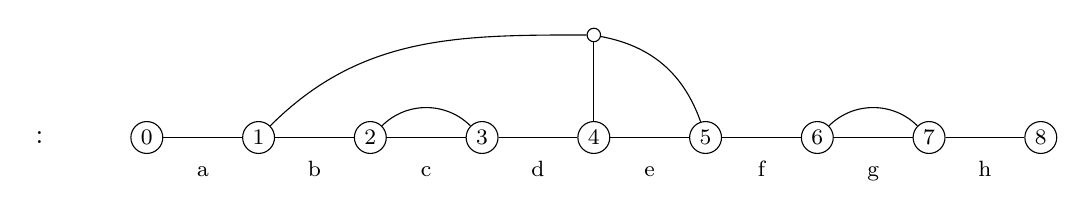
\begin{tikzpicture}
\tikzstyle{vertex}=[circle, draw, inner sep=0.5ex]
\footnotesize
\node (ci) {\normalsize :};
\node [vertex, right=of ci] (0) {0};
\foreach \n/\e in {1/a,2/b,3/c,4/d,5/e,6/f,7/g,8/h} {
  \pgfmathtruncatemacro{\left}{\n-1}
  \node [vertex] (\n) [right=of \left] {\n};
  \draw  (\left) -- node[below=5mm, anchor=base] {\e} (\n);
};

\node (x1) [above= of 4,vertex] {};
\draw (1) edge [in=180] (x1);
\draw (x1) edge (4)
  edge [bend left] (5);
\draw (2) edge [out =45] (3);

\draw (6) edge [out = 45] (7);
\end{tikzpicture}\\\vspace{5ex}
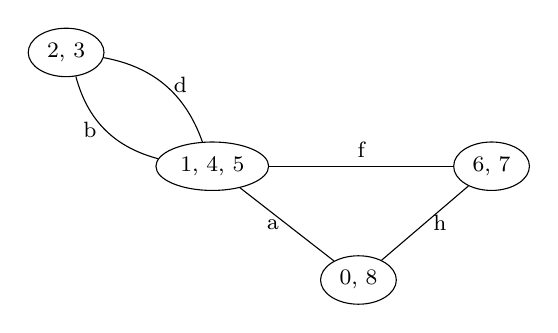
\begin{tikzpicture}
\footnotesize
\tikzstyle{blob}=[draw, ellipse]
\node (a) [blob] {0, 8};
\node (b) [blob, above right=of a] {6, 7};
\node (c) [blob, above left = of a] {1, 4, 5};
\node (d) [blob, above left = of c] {2, 3};

\draw (a) edge node [right] {h} (b)
  edge node [left] {a} (c);
\draw (c) edge [bend left] node [left] {b} (d)
  edge [bend right] node [right] {d} (d);
\draw (b) edge node [above] {f} (c);
\end{tikzpicture}
\caption{\label{fig:cactus} The segments attached to chain  and the corresponding part of the cactus. We first tentatively assign vertices 1--7 to the blob containing the endpoints  of . The top level cuts  are the pairs in the block . So we create a cycle with three edges and attach it to the blob containing 0 and 8. We move vertices 1--5 to the blob between  and , vertices 6--7 to the blob between  and , and keep vertices  and  in the parent blob. We then recurse into the first blob. The second level cuts are the pairs in the block . So we create a cycle with two edges and move vertices 2 and 3 to the new blob.}
\end{figure}

Graphs that contain nodes of degree two can be handled in the same way, if we add a cycle to each degree two node . This cycle creates a segment w.r.t.\ the chain to which  s-belongs and hence the algorithm correctly identifies the two incident edges as cut edges.





\begin{lemma} The above incremental procedure constructs a cactus representation of the 2-edge-cuts in  in linear time.
\end{lemma}
\begin{proof} Each vertex in  s-belongs to some chain. In the phase in which that chain is treated, all its vertices are added to a blob. Whenever we move a vertex to different blob, we remove it from its previous blob. Therefore each vertex of  is contained in exactly one blob.

Whenever we add edges to the cactus, we do so by adding a cycle that shares exactly one node with the existing cactus. Hence every edge in the cactus lies on exactly one cycle.

Let  be a 2-edge-cut in . The two edges must lie on a common cycle in the cactus, since the edges in the cactus are in one-to-one correspondence with edges of  and cutting a cycle in only one place cannot disconnect a graph. As the cycles of the cactus touch in at most one vertex,  and  are a cut in the cactus as well.

Conversely let ,  be a cut in the cactus and let ,  be the corresponding edges in . Then ,  must lie on some common cycle which, upon their removal, is split into two nonempty parts , and . Assume that  is still connected, then there must be a path from a vertex in the preimage of  to a vertex in the preimage of  in . This path must contain at least one edge  that does not participate in any 2-edge-cut, as otherwise it would be a path in the cactus as well. Moreover,  and  must lie in different blobs  and  of the cactus.

The one that was created last, say , must be different from the initial blob. Consider the time when  was created in the incremental construction of the cactus. We introduced a cycle to some preexisting blob  on which all edges were cut edges, in particular the two cut edges incident to . However, the edge  still connects  to the rest of graph, since  also exists at this time, a contradiction.
\end{proof}

By applying the techniques of this section, the certifying algorithm for -vertex-connectivity~\cite{Schmidt2013} (which is also based on chain decompositions) can be used to compute the -vertex-connected components of a graph. This has been conjectured in~\cite[p.\ 18]{Schmidt2010b} and yields a linear-time certifying algorithm to construct a SPQR-tree of a graph; we refer to~\cite{Hopcroft1973,Gutwenger2001} for details about -vertex-connected components and SPQR-trees. The full construction can be found in the appendix, section~\ref{3-Vertex Components}.

\section{Conclusion}\label{Conclusion}
We presented a certifying linear time algorithm for 3-edge-connectivity based
on chain decompositions of graphs. It is simple enough for use in a classroom setting and can serve as a gentle introduction to the certifying 3-vertex-connectivity algorithm of~\cite{Schmidt2013}. We also provide an implementation in Python, available at \url{https://github.com/adrianN/edge-connectivity}.

We also show how to extend the algorithm to construct and certify a cactus representation of all 2-edge-cuts in the graph. From this representation the 3-edge-connected components can be readily read off. The same techniques are used to find the 3-vertex-connected components using the algorithm from~\cite{Schmidt2013}, and thus present a certifying construction of SPQR-trees.

Mader's construction sequence is general enough to construct -edge-connected graphs for any , and can thus be used in certifying algorithms for larger . So far, though, it is unclear how to compute these more complicated construction sequences. We hope that the chain decomposition framework can be adapted to work in these cases too.




\begin{thebibliography}{10}

\bibitem{FormalVerification}
E.~Alkassar, S.~B\"ohme, K.~Mehlhorn, and Ch. Rizkallah.
\newblock A framework for the verification of certifying computations.
\newblock {\em Journal of Automated Reasoning (JAR)}, 52(3):241--273, 2014.

\bibitem{Bondy2008}
J.~A. Bondy and U.~S.~R. Murty.
\newblock {\em Graph Theory}.
\newblock Springer, 2008.

\bibitem{corcoran2006perfect}
J.~N. Corcoran, U.~Schneider, and H.-B. Sch{\"u}ttler.
\newblock Perfect stochastic summation in high order feynman graph expansions.
\newblock {\em International Journal of Modern Physics C}, 17(11):1527--1549,
  2006.

\bibitem{dehne2006cluster}
F.~Dehne, M.~Langston, X.~Luo, S.~Pitre, P.~Shaw, and Y.~Zhang.
\newblock The cluster editing problem: Implementations and experiments.
\newblock {\em Parameterized and Exact Computation}, pages 13--24, 2006.

\bibitem{Dinits-Karzanov-Lomonosov}
E.A. Dinits, A.V. Karzanov, and M.V. Lomonosov.
\newblock On the structure of a family of minimal weighted cuts in graphs.
\newblock In {\em Studies in Discrete Mathematics (in Russian)}, pages
  290--306. 1976.

\bibitem{Fleiner2009}
T.~Fleiner and A.~Frank.
\newblock A quick proof for the cactus representation of mincuts.
\newblock Technical Report QP-2009-03, Egerv{\'a}ry Research Group, Budapest,
  2009.

\bibitem{Gabow2000}
H.~N. Gabow.
\newblock Path-based depth-first search for strong and biconnected components.
\newblock {\em Inf. Process. Lett.}, 74(3-4):107--114, 2000.

\bibitem{Galil1991}
Z.~Galil and G.~F. Italiano.
\newblock Reducing edge connectivity to vertex connectivity.
\newblock {\em SIGACT News}, 22(1):57--61, 1991.

\bibitem{Gutwenger2001}
C.~Gutwenger and P.~Mutzel.
\newblock A linear time implementation of {SPQR}-trees.
\newblock In {\em Proceedings of the 8th International Symposium on Graph
  Drawing (GD'00)}, pages 77--90, 2001.

\bibitem{HT}
J.~Hopcroft and R.~Tarjan.
\newblock Efficient planarity testing.
\newblock {\em Journal of the ACM (JACM)}, 21(4):549--568, 1974.

\bibitem{Hopcroft1973}
J.~E. Hopcroft and R.~E. Tarjan.
\newblock Dividing a graph into triconnected components.
\newblock {\em SIAM J. Comput.}, 2(3):135--158, 1973.

\bibitem{Karger2000}
D.~R. Karger.
\newblock Minimum cuts in near-linear time.
\newblock {\em J. ACM}, 47(1):46--76, 2000.

\bibitem{Linial1988}
N.~Linial, L.~Lov{\'a}sz, and A.~Wigderson.
\newblock Rubber bands, convex embeddings and graph connectivity.
\newblock {\em Combinatorica}, 8(1):91--102, 1988.

\bibitem{Lovasz1985}
L.~Lov\'asz.
\newblock Computing ears and branchings in parallel.
\newblock In {\em Proceedings of the 26th Annual Symposium on Foundations of
  Computer Science (FOCS'85)}, 1985.

\bibitem{Mader1978}
W.~Mader.
\newblock A reduction method for edge-connectivity in graphs.
\newblock In B.~Bollob\'as, editor, {\em Advances in Graph Theory}, volume~3 of
  {\em Annals of Discrete Mathematics}, pages 145--164. 1978.

\bibitem{McConnell2011}
R.~M. McConnell, K.~Mehlhorn, S.~N\"aher, and P.~Schweitzer.
\newblock Certifying algorithms.
\newblock {\em Computer Science Review}, 5(2):119--161, 2011.

\bibitem{Me3}
K.~Mehlhorn.
\newblock Nearly optimal binary search trees.
\newblock {\em Acta Informatica}, 5:287--295, 1975.

\bibitem{Mehlhorn1999}
K.~Mehlhorn, S.~N{\"a}her, and C.~Uhrig.
\newblock {\em The {LEDA} Platform of Combinatorial and Geometric Computing}.
\newblock Cambridge University Press, 1999.

\bibitem{Nagamochi1992a}
H.~Nagamochi and T.~Ibaraki.
\newblock A linear time algorithm for computing 3-edge-connected components in
  a multigraph.
\newblock {\em Japan Journal of Industrial and Applied Mathematics},
  9:163--180, 1992.

\bibitem{Nagamochi-Ibaraki-Book}
H.~Nagamochi and T.~Ibaraki.
\newblock {\em Algorithmic Aspects of Graph Connectivity (Encyclopedia of
  Mathematics and its Applications)}.
\newblock Cambridge University Press, 2008.

\bibitem{Neumann2011}
A.~Neumann.
\newblock Implementation of {S}chmidt's algorithm for certifying
  triconnectivity testing.
\newblock Master's thesis, Universit\"at des Saarlandes and Graduate School of
  CS, Germany, 2011.

\bibitem{Verification-CertComps-AutoCorres-Simpl}
Lars Noschinski, Christine Rizkallah, and Kurt Mehlhorn.
\newblock Verification of certifying computations through {A}utocorres and
  {S}impl.
\newblock In {\em NASA Formal Methods}, volume 8430 of {\em LNCS}, pages
  46--61. 2014.

\bibitem{Olariu1996}
S.~Olariu and A.~Y. Zomaya.
\newblock A time- and cost-optimal algorithm for interlocking sets -- {W}ith
  applications.
\newblock {\em IEEE Trans. Parallel Distrib. Syst.}, 7(10):1009--1025, 1996.

\bibitem{Ramachandran1993}
V.~Ramachandran.
\newblock Parallel open ear decomposition with applications to graph
  biconnectivity and triconnectivity.
\newblock In {\em Synthesis of Parallel Algorithms}, pages 275--340, 1993.

\bibitem{Schmidt2010b}
J.~M. Schmidt.
\newblock Contractions, removals and certifying 3-connectivity in linear time.
\newblock Tech. Report B 10-04, Freie Universit\"at Berlin, Germany, May 2010.

\bibitem{Schmidt2013}
J.~M. Schmidt.
\newblock Contractions, removals and certifying 3-connectivity in linear time.
\newblock {\em SIAM Journal on Computing}, 42(2):494--535, 2013.

\bibitem{Schmidt2013a}
J.~M. Schmidt.
\newblock A simple test on 2-vertex- and 2-edge-connectivity.
\newblock {\em Information Processing Letters}, 113(7):241--244, 2013.

\bibitem{Taoka1992}
S.~Taoka, T.~Watanabe, and K.~Onaga.
\newblock A linear time algorithm for computing all 3-edge-connected components
  of a multigraph.
\newblock {\em IEICE Trans. Fundamentals E75}, 3:410--424, 1992.

\bibitem{Tsin2007}
Y.~H. Tsin.
\newblock A simple 3-edge-connected component algorithm.
\newblock {\em Theor. Comp. Sys.}, 40(2):125--142, 2007.

\bibitem{Tsin2009}
Y.~H. Tsin.
\newblock Yet another optimal algorithm for 3-edge-connectivity.
\newblock {\em J. of Discrete Algorithms}, 7(1):130--146, 2009.

\bibitem{Vo1983}
K.-P. Vo.
\newblock Finding triconnected components of graphs.
\newblock {\em Linear and Multilinear Algebra}, 13:143--165, 1983.

\bibitem{Vo1983a}
K.-P. Vo.
\newblock Segment graphs, depth-first cycle bases, 3-connectivity, and
  planarity of graphs.
\newblock {\em Linear and Multilinear Algebra}, 13:119--141, 1983.

\end{thebibliography}



\appendix

\section{Computing a Spanning Subgraph of an Overlap Graph}

We first assume that all endpoints are pairwise distinct. We will later show how to remove this assumption by perturbation.

For every interval  define its set of left and right neighbors:

If the set of left neighbors is nonempty, let the interval  with the rightmost right endpoint be the immediate left neighbor of . Similarly, if the set of right neighbors is nonempty, the immediate right neighbor of  is the interval in  with the leftmost left endpoint.

\begin{lemma} The graph  formed by connecting each interval to its immediate left and right neighbor (if any) forms a spanning subgraph of the overlap graph  and has exactly the same connected components.
\end{lemma}
\begin{proof} Clearly, every edge of  is also an edge of  and hence
  connected components of  are subsets of connected components of .

For the other direction, assume  and  are overlapping intervals that are not connected in . Then , where  and . Let  be such that  is the immediate right neighbor of  for all . Consider the last  in this sequence such that ; clearly, such an interval exists, as  is such an interval. Then  is a right neighbor of , but not the immediate right neighbor of , as otherwise  and  would be connected in . Hence, the immediate right neighbor  of  exists, is different from , and must contain . Thus

Starting from  and going to immediate left neighbors, we obtain in the same fashion an interval  with

We conclude that  and  overlap, but are not connected in . 

Consider now a particular choice for the overlapping intervals  and . We choose them such that the left endpoint of  is as small as possible. However, the left endpoint of  is to the left of the left endpoint of , and we have derived a contradiction. \qed
\end{proof}

\begin{algorithm}[t]
\caption{Finding a spanning forest of a overlap graph}
\label{alg:spanning_tree}
\begin{algorithmic}
	\Procedure{SP}{}
	\State stack = [\,]
	\State sort  lexicographically in descending order
	\For{ in }
	  \While{stack not empty and  top(stack) right endpoint}
	    \State pop(stack)
	  \EndWhile
	  \If{stack not empty and  top(stack) left endpoint}
	    \State connect , top(stack)
	  \EndIf
	  \State push(stack, )
	\EndFor
	\State stack = [\,]
	\State sort  lexicographically in ascending order where the key for  is 
	\For{ in }
	  \While{stack not empty and <top(stack) left endpoint}
	    \State pop(stack)
	  \EndWhile
	  \If{stack not empty and  top(stack) right endpoint}
	    \State connect , top(stack)
	  \EndIf
	  \State push(stack, )
	\EndFor
	\EndProcedure
\end{algorithmic}
\end{algorithm}

It is easy to determine all immediate right neighbors by a linear time sweep over all intervals. We sort the intervals in decreasing order of left endpoint and then sweep over the intervals starting with the interval with rightmost left endpoint. We maintain a stack  of intervals, initially empty. If  are the intervals on the stack with  being on the top of the stack, then  and ,  is the last interval processed, and  is the immediate right neighbor of  if  has right neighbors. If  does not have right neighbors, . Let  be the next interval to be processed. Its immediate right neighbor is the topmost interval  on the stack with  (if any). Hence we pop intervals  from the stack while  and then connect  to the topmost interval if , and push . The determination of immediate left neighbors is symmetric.

It remains to deal with intervals with equal endpoints. We do so by perturbation. It is easy to see that the following rules preserve the reachability by overlaps and eliminate equal endpoints. E.g., in (4), the two intervals are forced to overlap, so reaching one of the two intervals gives a path to the other; the same reasoning motivates (2) and (3).
\begin{compactenum}[(1)]
\item if a left and a right endpoint are at the same coordinate, then the left endpoint is smaller than the right endpoint.
\item if two left endpoints are equal, the one belonging to the shorter interval is smaller.
\item if two right endpoints are equal, the one belonging to the shorter interval is larger.
\item if two intervals are equal, one is slightly shifted to the right.
\end{compactenum}
In other words, the endpoints of an interval  are replaced by  and  and comparisons are lexicographic. The perturbation need not be made explicitly, it can be incorporated into the sorting order and the conditions under which edges are added, as described in Algorithm~\ref{alg:spanning_tree}.



\section{Computing all 3-Vertex-Connected Components}\label{3-Vertex Components}

A pair of vertices  is a separation pair of  if  is disconnected. Similar to the edge-connectivity case, it suffices to compute all vertices that are contained in separation pairs of  in order to compute all -vertex-connected components of . We assume that  is -vertex-connected and has minimum degree .

For a rooted tree  of  and a vertex , let  be the subtree of  rooted at . The following lemmas show that separation pairs can only occur in chains. Weaker variants of Lemma~\ref{lem:separationpair} can be found in~\cite{Hopcroft1973,Vo1983,Vo1983a}.



\begin{lemma}\label{lem:separationpair}
Let  be a DFS-tree of a -connected graph  and  be a chain decomposition of . For every separation pair  of ,  and  are contained in a common chain .
\end{lemma}
\begin{proof} The following simple observation will be useful. Let  be the root of  and let  be any vertex. Then for every , there is a path  from  to a vertex  such that  consists only of vertices in .


We first prove that  and  are \emph{comparable} in , i.e., contained in a leaf-to-root path of . Assume they are not. Then  consists of at most three connected components: one connected component containing the least common ancestor of  and  in , and the at most two connected components that contain the proper descendants of  and , respectively. According to the observation above,
these components coincide, contradicting that  is a separation pair.

Let  be the child of  in  that lies on the path . Clearly, if , the chain containing the edge  is a common chain containing  and . Otherwise, . If , then there is a back-edge  such that , according to the fact that  is connected by  and due to the observation above. This back-edge  implies that the first chain  that traverses a vertex of  starts at  and, hence, contains  and .

In the remaining case,  and . Let  be a back-edge that connects an ancestor  of  with a descendant  of  (possibly  itself) such that  is minimal; this edge  exists, since  is -vertex-connected. According to~\cite{Schmidt2013a},  is the only cycle in  and it follows that . If , the first chain  in  that contains such a back-edge contains  and  and, hence, satisfies the claim. Otherwise,  is a vertex in . Due to the back-edge ,  is contained in one connected component of . According to the observation above (applied on ),  can form a separation pair only if  has a child  such that all back-edges that end in  start either in  or at . Since  is -connected, there must be a back-edge from  to . The first chain  in  containing such a back-edge gives the claim, as it contains  and .
\end{proof}

Similar to edge-connectivity, the connected components of the overlap graph for  represent all vertices in separation pairs that are contained in . The connected components of the overlap graph can be computed efficiently~\cite[Lemma~51]{Schmidt2013}. After finding all these vertices for , a simple modification allows the algorithm in~\cite[p.\ 508]{Schmidt2013} to continue, ignoring all previously found separation pairs: For every separation pair , , that has been found when processing , there is a vertex  strictly between  and  in . Furthermore, by doing a preprocessing~\cite[Property~B, p.\ 508]{Schmidt2013} one can assume that  also has an inner vertex . We eliminate every separation pair  after processing  by simply adding the new back-edge  to . As the new chain containing  is just an edge, this does not harm future processing steps.

According to Lemma~\ref{lem:separationpair}, this gives all vertices in the graph that are contained in separation pairs. The -vertex-connected components can then be computed in linear time by iteratively splitting separation pairs and gluing together certain remaining structures, as shown in~\cite{Hopcroft1973,Gutwenger2001}.



\end{document}